\chapter{Simulations}

Simuler des images réalistes est un enjeu important en imagerie médicale. Le fait d'avoir accès à la vérité terrain, contrairement à la routine clinique, permet de valider des hypothèses de manière beaucoup plus fine. De plus, avec l'augmentation des performances de ordinateurs et l'accès à des centres de calculs, il devient possible de créer des bases de données de patients de plus en plus importantes et réalistes.

	\section{principe des simulations}

		\subsection{analytiques}

Les simulateurs Analytiques ne simulent pas de manière réaliste le déplacement des particules mais  utilisent des approximation fortes pour résoudre les problèmes de manière analytiques..

Dans le cas de l'imagerie TEP, la simulation analytique revient à réaliser des projections du volume TEP dans l'espace du sinogramme. Ce sinogramme est ensuite bruité et modifié pour prendre en compte les effets des coïncidences aléatoires, ou des photons diffusés. L'efficacité des détecteurs est aussi prise en compte, tout comme les effets de l'atténuation. 

La reconstruction est ensuite réalisée de manière classique à l'aide des algorithmes de reconstruction TEP.


Cependant, bien que ce type de simulateur est extrêmement rapide, les images générées ne parviennent pas à reproduire de manière parfaite les différentes limitations 

		\subsection{monte carlo}

Les simulations Monte-Carlo vont avoir une approche probabiliste en modélisant la trajectoire de chaque photon indépendamment. Le nom de Monte-Carlo fait allusion aux jeux de hasards pratiqués dans la ville du même nom.

Dans le cadre de l'imagerie TEP, le modèle probabiliste est appliqué depuis l'émission puis le parcours du positon, l'annihilation, ainsi que les interactions et la probabilité de détection des photons dans les détecteurs.

La génération et le suivi de chaque photon ainsi que de chaque désintégration prennent un temps extrêmement important, amplifié par le fait que deux désintégrations successives dans des organes différents peuvent amener à une coïncidence fortuite sous certaines conditions. Il faut aussi prendre en compte les limitations de l'électronique, ce qui amène à des temps de simulation prohibitifs.

		\subsection{MC accélérés}

Les simulateurs Monte-Carole accéléré utilisent des heuristiques pour accélérer les calculs, notamment en réalisant des calculs préliminaires afin de simplifier les simulations futures. 

La séparation des simulations entre les coïncidences directes et les diffusés, à l’aide des statistiques crées précédemment, permet encore d’accélérer les calculs.

	\section{simulateurs disponibles}

De nombreux simulateurs ont été développés par la communauté. Ils sont souvent développés à partir d'une librairie dédiée au calculs de trajectoires de particules, comme GATE~\cite{jan2004gate}, qui se base sur le jeu d'outils de simulation d'interactions particule/matière geant4~\cite{allison2006geant4}, le simulateur Penelo-PET\cite{espana2009penelopet} basé sur la librairie de simulation  PENELOPE,\cite{salvat2006penelope}, ou encore EGS-PET. L’université de Washington développe le simulateur monte-carlo simSET ainsi que le simulateur analytique ASIM. 

Nous avons utilisé PET-SORTEO, car il a été développé depuis le début pour réduire la vitesse de calculs et profiter de la parallélisassion offerte par les centres de calculs. De plus, nous avons réalisé la première version de la base de donnée OncoPET\_BD~\cite{tomei2010oncopet_db} sur ce simulateur, ce qui permet de capitaliser sur l’expérience déjà acquise avec ce simulateur. 

	\section{processus de simulation avec SORTEO}

Pour reproduire les données fournies par les systèmes cliniques TEP, les simulateurs Monte-Carlo simulent les désintégrations une par une et suivent les sous-produits dans les tissus jusqu'aux détecteurs. Étant donné qu'un examen TEP génère plusieurs millions de désintégrations, les temps de simulations deviennent très rapidement insurmontables. PET-SORTEO dispose de plusieurs heuristiques qui permettent d'accélérer les simulations, notamment en séparant les simulations des différents types de coïncidences en fonction de statistiques estimées au début de la simulation. Cependant il faut tout de même plusieurs dizaines d'heures pour simuler une image.

La première étape consiste à rédiger un fichier de \emph{protocole} récapitulant les activités et l'atténuation présentes dans les différentes régions du fantôme. Les paramètres du scanner (modèle, type d'acquisition) sont aussi définis, tout le format de sortie

Il est possible de définir deux fantômes différents pour l'émission et l'atténuation. Ces fantômes voxeliques doivent être fournis au format ECAT (développé par Siemens) et sont des cartes de labels auxquels seront associés les activités ou les atténuations du fichier protocole.

Ensuite, la première partie de la simulation est utilisée pour déterminer un ensemble de probabilités permettant d'accélérer les calculs futurs. Pour cela, il réalise des simulation monte-carlo complètes pour chaque label avec un faible nombre de photons. Cela permet de calculer plusieurs grandeurs tels que la probabilité de détection des photons pour chaque couple (label, détecteur) en prenant en compte les phénomènes physiques, ou encore la probabilité de détection en coïncidence des deux photons émis lors d'une désintégration pour chaque label.

La seconde partie de la simulation corresponds à la réalisation de l'examen proprement dit. C'est à cette étape que seront simulées les coïncidences vraies, diffusées ou non. Chaque coïncidence de chaque label est simulée une par une, et le trajet de chaque photon est calculé indépendamment. Si un des photons est absorbé ou que son énergie est en dehors de celle de la fenêtre de sensibilité, alors la paire est considérée comme perdue le programme passe à la désintégration suivante. A cette étape, le programme prend en compte les temps mort (limitation de l'électronique qui ne peut pas prendre en compte un trop grand nombre de photons en même temps), qui dépend de l'activité. Il est intéressant de noter que grâce aux statistiques estimées à la première étape, la trajectoire de certains photons n'est pas calculée car le simulateur considère qu'ils font partie des ``pertes``. C'est ce qui permet de réaliser les calculs très rapidement par rapport aux simulations monte-carlo classiques.

La dernière étape est utilisée pour simuler les coïncidences aléatoires, qui seront ajoutées aux données précédentes.


Le modèle utilisé par SORTEO est un compromis intéressant entre le réalisme apporté par les méthodes de Monte-Carlo et les performances apportées par les techniques de pré-calculs de statistiques ainsi que de séparation du calcul des coïncidences directes et fortuites. L'auteur annonce que toutes les sources majeures de bruit et de biais sont prises en compte.

Le simulateur PET-SORTEO a été validé pour le simulateur Ecat Exact HR+~\cite{reilhac2004pet} ainsi que pour la plateforme PET Philips Allegro, qui est incluse dans les scanner TEP/TDM Gemini.


	\section{Contribution à PET-SORTEO}

Lors de ma thèse j'ai effectué plusieurs contributions au code de PET-SORTEO, notamment au niveau de la partie découpage des tâches pour l'exécution en centre de calcul, et au niveau de l'adaptation du programme aux données séquences.

\subsection{Adaptation pour l'exécution sur centre de calcul}

Le code original de SORTEO était adapté à une exécution sur des centres de calculs de petite taille, où la communication entre les processus n’est pas limitée. Cependant, étant donné les volumes de calculs représentés par nos simulations, nous avons fait appel au centre de calcul de l'in2p3 (Institut national de physique nucléaire et de physique des particules).

Ce centre de calcul regroupe plus de 1300 machines totalisant plus de 17000 cœurs, ainsi que 13 Petaoctets de stockage sur disques en 2011. Les technologies mises en places sont spécialisées pour gérer cette quantité de données, ce qui représente des limitations quand aux techniques employées par les logiciels.

Par exemple, les différents processus du simulateur PET-SORTEO dialoguaient à travers des fichiers partagés. Cela engendrait des problèmes de saturation de la bande passante entre les nœuds. J'ai donc réalisé des modifications en profondeur du code pour séparer le simulateur en plusieurs entités, chacune réalisant une seule partie du travail :

    \begin{enumerate}
        \item Estimation des paramètres nécessaires à la simulation accélérée par simulation Monte-Carlo pur (lancé pour chaque processus)
        \item Combinaison des résultats Monte-Carlo
        \item Simulation simplifiée des désintégrations (lancé pour chaque processus)
        \item Combinaison des désintégrations détectées pour chaque processus dans un seul fichier de données
    \end{enumerate}

Ensuite, un ensemble de scripts est réalisé pour automatiser les opérations de combinaison des résultats et de calcul des statistiques, puis pour relancer les simulations des coïncidences vraies et fortuites. Une dernière étape consiste à réassembler les détections pour générer les données liste.

\subsection{Sortie en mode Séquence}

Bien que le code original permettait de spécifier un format de sortie, en pratique seul le format sinogramme était pris en compte. 

En effet, le code original ne permettait pas la sauvegarde de l'information temporelle de chaque évènement détecté. Or cette information est nécessaire aux méthodes de correction du mouvement du mouvement respiratoire. 

Nous avons donc repris un travail commencé par des étudiants en stage pour adapter PET-SORTEO au nouveau format. Nous avons repris le format LMF développé pour la plateforme micro-PET pour générer les données car ce format de données est simple à utiliser. 


\section{Reconstruction des images}

Nous avons utilisé le logiciel de reconstruction fourni par le LaTIM dans le cadre d'un partenariat, crée et utilisé par Frédéric Lamare pour ses travaux sur la correction du mouvement respiratoire~\cite{lamare2007list}.

Il est capable de reconstruire les images acquises en données séquentielles à l'aide de l'algorithme OPL-EM décrit en \ref{lab:OPLEM}. La reconstruction permet de prends en compte la correction de l'atténuation, mais ne permet pas la correction des coïncidences aléatoires ni des diffusés. Nous avons donc choisit de simplifier le problème en considérant que la correction de ces deux effets était parfaite, en n'incluant pas dans les données séquentielles les photons diffusés ou les coïncidences aléatoires.

Nous avons choisit de corriger les images en utilisant la méthode de correction post reconstruction décrite en \ref{lab:corrPostRecon} ainsi que la correction par modification de la matrice système décrite en \ref{lab:corrMatSyst}. La première est déjà implémentée sur les imageur GE (technologie motionFree), tandis que la seconde est activement étudiée en recherche. 




\subsection{Gestion des lits}

Le découpage des simulations en lits est nécessaire pour simuler de manière réaliste des acquisitions médicales. Or le logiciel de reconstruction avec correction de mouvement ne prenait pas en compte la possibilité de découper les images en lits.

Nous avons donc modifié le logiciel pour pouvoir prendre en compte des champs de mouvements de taille plus importante que celle d'un lit. En pratique le lit à recaler est insérée dans une image complète qui sera déformée, puis le lit concerné sera extrait pour continuer la reconstruction


\subsection{Paramètres de reconstruction}

L'un des paramètres principaux à prendre en compte lors de la reconstruction est le nombre d'itérations de la méthode~\ref{fig:evolRecon}. Nous avons choisit d'utiliser une méthode basée sur les sous-ensembles car elle permet d'accélérer de manière significative les reconstructions. Nous avons choisit de travailler avec 5 sous-ensembles.

\begin{figure}
\centering
\begin{tabular}{|c|c|c|c|}
 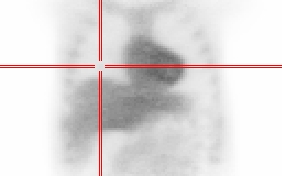
\includegraphics[width=3cm]{images/ite1} & 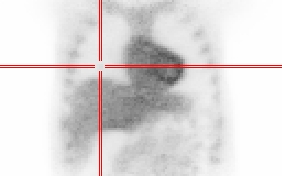
\includegraphics[width=3cm]{images/ite3} & 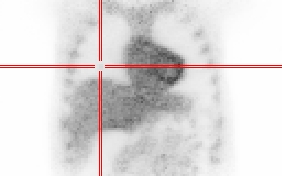
\includegraphics[width=3cm]{images/ite5} & 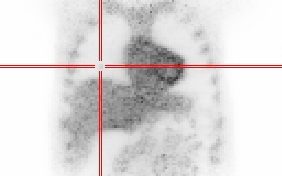
\includegraphics[width=3cm]{images/ite7} \\
Itération 1  & Itération 3 & Itération 5 & Itération 7 \\
\hline
 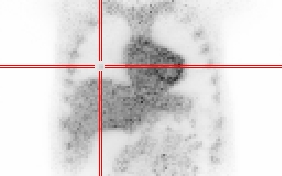
\includegraphics[width=3cm]{images/ite9} & 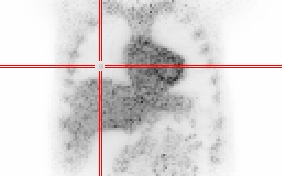
\includegraphics[width=3cm]{images/ite11} & 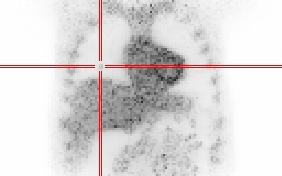
\includegraphics[width=3cm]{images/ite13} &  \\
Itération 9  & Itération 11 & Itération 13 &\\
\end{tabular}

\caption[Illustration de l'évolution des lésions en fonction du nombre d'itérations]{Illustration de l'évolution des images en fonction du nombre d'itérations. Une lésion est présente au centre de la croix rouge.}
\label{fig:evolRecon}
\end{figure}

L'optimisation du nombre d'itérations totales est réalisée en utilisant le rapport contraste sur bruit~\cite{takahara2004diffusion}, défini comme suit :

\begin{equation}
 CSB = \frac{µ_{signal} - µ_{fond}}{\sqrt{\sigma_0}}
\end{equation}

Avec $µ_{signal}$ et $µ_{fond}$ représentant respectivement l'activité moyenne d'une zone d'intérêt centrée sur une lésion et l'activité moyenne d'une zone saine. $\sigma_0$ représente la variance du bruit. Dans notre cas elle est évaluée dans une zone saine de l'organe où se trouve la tumeur. Appliquée aux lésions, cette métrique a l'avantage de permettre une représentation rapide de l'évolution du contraste entre la lésion et le fond, tout en prenant en compte la montée en bruit.

L'évaluation du rapport contraste sur bruit est réalisé pour toutes les lésions l'un des modèles en fonction du nombre d'itérations complètes sur le Foie (6 lésions) et le Poumon (6 lésions).

Les résultats sont présentés dans la figure \ref{fig:CNRFoie} pour le Foie et \ref{fig:CNRPoumon} pour le poumon.

\begin{figure}
\centering
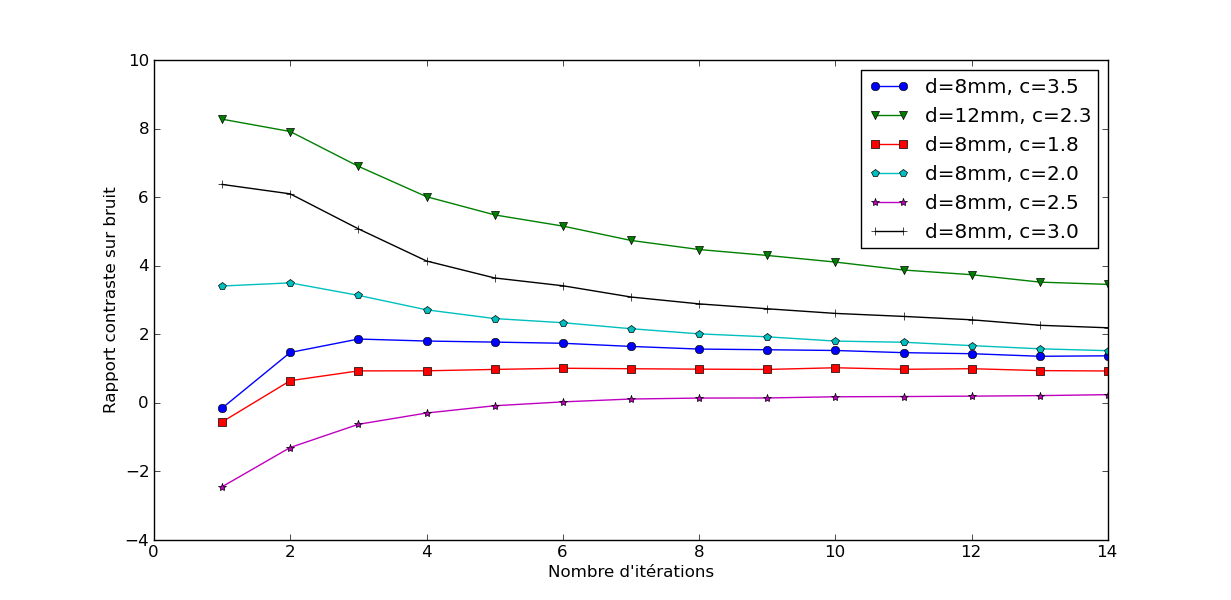
\includegraphics[width=17cm]{images/CNRFoie}
\caption[Evaluation du rapport Contraste sur bruit des lésions du foie en fonction du nombre d'itérations]{Evaluation du rapport Contraste sur bruit des lésions du foie en fonction du nombre d'itérations : sont indiqués pour chaque lésion le niveau de contraste ainsi que le diamètre de la lésion}
\label{fig:CNRFoie}
\end{figure}


\begin{figure}
\centering
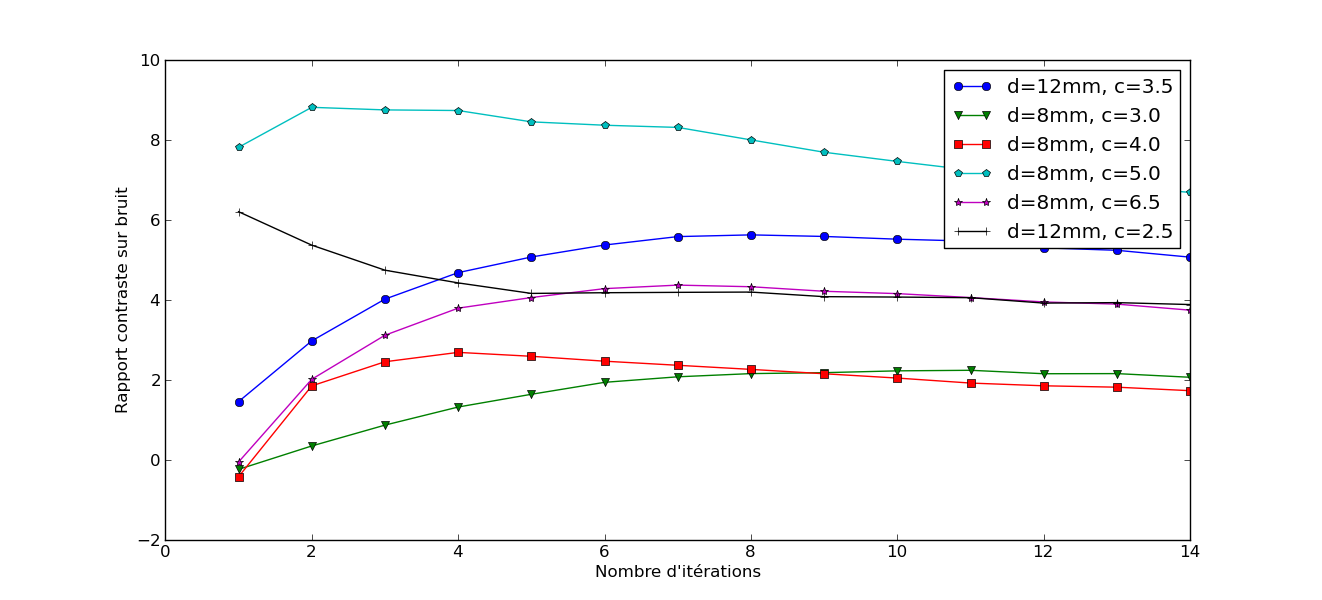
\includegraphics[width=17cm]{images/CNRPoumon}
\caption[Evaluation du rapport Contraste sur bruit des lésions du poumon en fonction du nombre d'itérations]{Evaluation du rapport Contraste sur bruit des lésions du poumon en fonction du nombre d'itérations : sont indiqués pour chaque lésion le niveau de contraste ainsi que le diamètre de la lésion}
\label{fig:CNRPoumon}
\end{figure}

La première chose que l'on peut observer est que certaines courbes sont strictement descendantes, surtout dans le foie. Cela s'explique par le fait que le niveau de bruit augmente beaucoup plus rapidement que la différence d'activité entre le signal et le fond. Cependant, les lésions concernées ont toutes un contraste très élevé, ce qui les rend plus facilement détectables. Pour les autres, par contre, on peut voir que l'optimum des lésions du foie est situé autour de 4 itérations, suivi par un plateau, tandis que l'optimum des lésions du poumon est plus proche de 8 itérations complètes.

La lésion du foie ayant un niveau contraste 3 et un diamètre de 8mm a une valeur de rapport contraste sur bruit négative. Cela s'explique par le fait que pour les premières itérations, une faible différence d'activité négative peut être fortement accentuée par l'écart type qui est très faible. De la même manière, pour les itérations suivantes, l'activité de cette lésion redevient supérieure à celle du fond, mais l'écart-type du bruit devient plus important, ce qui fait que le rapport est proche de 0.

Nous avons choisit de réaliser les reconstructions avec 8 itérations car nous avons montré que ce nombre d'itérations est optimal pour les lésions du poumon, et ne pénalise pas trop les lésions du foie.



\section{Estimation de mouvement}

L'estimation de mouvement est réalisée uniquement à partir des données TEP et des informations de synchronisation respiratoire. 

\subsection{Principe de l'estimation de mouvement}

L'estimation de mouvement est réalisée selon le principe énoncé en~\ref{lab:estimMvtTEP4D} :
\begin{enumerate}
 \item Les données simulées des 4 cycles sont additionnées pour chaque instant respiratoire.
 \item Les images correspondant à chaque instant du cycle respiratoire sont reconstruites à partir de ces données en utilisant l'algorithme OPL-EM.
 \item Les 8 images générées sont utilisées pour calculer le mouvement respiratoire : Les images des temps 2 à 8 sont recalées sur l'image de référence (numéro 1), ce qui associe à chaque instant respiratoire un champ de déformation.
\end{enumerate}


Le champ de mouvement est estimé en utilisant un code fourni par Philips, correspondant à une implémentation de recalage par B-splines. La transformation $g_t(x)$ utilisée pour associer les images temporelle  $f(x,t)$ (pour t allant de 2 à 8) avec l'image de référence $f(x,0)$, est représentée de la manière suivante :

\begin{equation}
  g_t(x)=x + \sum\limits_{j\in \mathbb{Z}^N} c_j \beta^n \left( \frac{x}{h-j} \right)
\end{equation}

avec $\beta^n$ qui représente la fonction B-spline de degré $n$, $j$ les indices des positions de la grille. $h$ correspond à l'espacement entre les points de la grille et $r$. A chaque point de la grille corresponds un coefficient associé nommé $c_j$ qui représente l'apport de la B-spline correspondante and le signal final.

Les meilleurs coefficients $c_j$ sont obtenus à l'aide d'une optimisation multi-échelle. Nous avons utilisé 3 niveaux, en réalisant l'optimisation par gradient conjugué par la méthode de Polak-Ribière~\cite{polak1969note}. La métrique utilisée pour comparer performance est la somme des différences au carré. 


\subsection{Paramètres de l'estimation de mouvement}

Les images correspondant à chaque instant respiratoire sont reconstruites séparément, avec des paramètres différents de ceux utilisés pour reconstruire les images complètes. En effet, la quantité de données disponible pour la reconstruction est 8 fois plus faible que celle utilisée pour réaliser les reconstructions d'images complètes. De plus, nous cherchons à optimiser la qualité de l'estimation de mouvement. C'est pour ces raisons que nous avons réalisé une autre étude pour estimer les paramètres de reconstruction optimaux. 

Pour évaluer la performance de chaque jeu de paramètre, nous avons utilisé la vérité terrain pour créer une image d'évaluation pour l'image de référence, ainsi qu'une autre pour l'image ``respirante``. Les images d'évaluations sont crées à partir des fantômes de référence en assignant aux organes étudiés (foie et poumon) une valeur de 1, et une valeur plus importante pour les lésions, comme indiqué dans la figure~\ref{lab:illustrationRecalage}.a). 

\begin{figure}
\centering
\begin{tabular}{c c}
	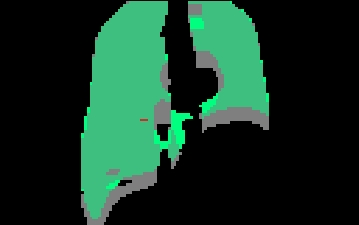
\includegraphics[width=5cm]{images/sansCorrection} & 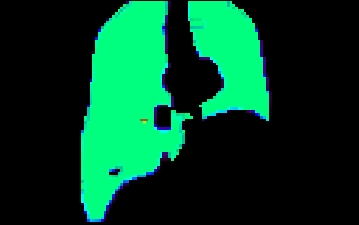
\includegraphics[width=5cm]{images/avecCorrection} \\
	a) Cartes non recalées				& b) Cartes recalées
\end{tabular}
\caption[Illustration du recalage obtenu]{Illustration de la pertinence du recalage obtenu à partir de l'estimation de mouvement réalisée sur les images. En vert l'image de référence et en gris l'image correspondant au temps correspondant à la différence la plus importante. }
\label{lab:illustrationRecalage}
\end{figure}

L'image d'évaluation correspondant à l'image ''respirante`` est alors recalées sur l'image de référence à l'aide du champ de mouvement élastique calculé précédemment. J'évalue ensuite la qualité du recalage en réalisant une somme des différences au carré entre les deux images d'évaluation~\ref{lab:illustrationRecalage}.b).


\subsubsection{Optimisation des paramètres de reconstruction}

Nous avons évalué la performance des reconstructions pour les paramètres suivants :
\begin{description}
 \item[Nombre d'itérations complètes :] Le nombre de sous-ensembles est toujours de 5, mais nous faisons varier le nombre d'itérations complètes de 1 à 7, ce qui représente un nombre d'itérations totales de 5 à 40.
 \item[Présence ou absence de régularisation pendant la reconstruction :] Une régularisation de 6 mm  est appliquée ou non à chaque itération complète.
\end{description}

Les résultats sont présentés dans la figure~\ref{lab:perfsFctIterReg}. Ils montrent clairement que la régularisation entraîne une amélioration des performances, et que la meilleure estimation de mouvement est réalisée pour une reconstruction de 3 itérations complètes avec 5 sous-ensembles. Nous avons utilisé une grille de $3 \times 3 \times 5$ noeuds.

\begin{figure}
\centering
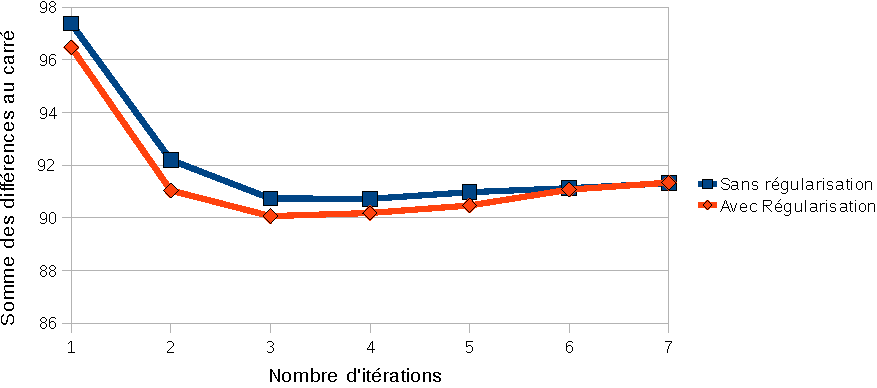
\includegraphics[width=10cm]{images/perfsRecalageFctIter_crop}
\caption[Performances de l'estimation de mouvement en fonction de la régularisation]{Performances de l'estimation de mouvement en fonction du nombre d'itérations complètes de la reconstruction selon la présence ou l'absence de régularisation pendant la reconstruction. Plus la valeur en ordonnées (mesure de différence) est faible, meilleure et la performance}
\label{lab:perfsFctIterReg}
\end{figure}

\subsubsection{paramètres de l'estimation de mouvement}


L'échantillonnage spatial utilisé pour l'estimation de mouvement doit aussi être évalué. En effet, si l'espacement entre les nœuds de contrôle est trop important, les mouvements locaux vont se parasiter et le résultat ne sera pas valide. De la même manière, en cas d'espacement trop faible, la nature extrêmement bruitée des images va engendrer des micro-mouvements parasites locaux.

C'est pour cela que nous avons mené une seconde étude paramétrique pour rechercher le nombre de nœuds idéal. L'étude a été réalisée en reconstruisant les images à l'aide des paramètres définis précédemment.

Nous avons évalué les performances de l'estimation de mouvement pour le nombre de nœuds suivants selon les axes X, Y puis Z :

\begin{itemize}
 \item $2 \times 2 \times 2$
 \item $3 \times 3 \times 5$
 \item $5 \times 5 \times 10$
\end{itemize}

Les résultats sont présentés dans la figure~\ref{fig:perfsFctIterTaille}

\begin{figure}
\centering
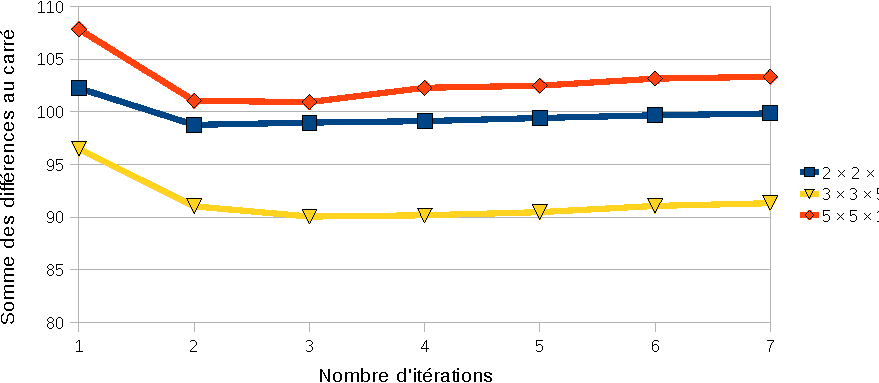
\includegraphics[width=10cm]{images/perfsRecalageFctIter-grid_crop}
\caption[Performances de l'estimation de mouvement en fonction de la taille de la grille de recherche]{Performances de l'estimation de mouvement en fonction du nombre d'itérations complètes de la reconstruction selon la taille de la grille utilisée pour l'estimation de mouvement}
\label{fig:perfsFctIterTaille}
\end{figure}

Les résultats nous montrent que les meilleures performances sont obtenues pour la configuration $3 \times 3 \times 5$, qui sont systématiquement meilleurs quelques soit le nombre d’itérations.


